\documentclass[conference]{IEEEtran}
\IEEEoverridecommandlockouts
\usepackage{cite}
\usepackage{amsmath,amssymb,amsfonts}
\usepackage{algorithmic}
\usepackage{graphicx}
\usepackage{textcomp}
\usepackage{xcolor}
\def\BibTeX{{\rm B\kern-.05em{\sc i\kern-.025em b}\kern-.08em
    T\kern-.1667em\lower.7ex\hbox{E}\kern-.125emX}}

\begin{document}

% Header
\title{RISK-VI Case Study\\}
\author{\IEEEauthorblockN{Jonathan Wang}
\IEEEauthorblockA{\textit{Electrical and Computer Engineering} \\
\textit{University of Utah}\\
Salt Lake City, United States \\
u1306458@umail.utah.edu}
}
\maketitle

% Abstract
\begin{abstract}
RISK-V FPGAs are attracting developers worldwide due to their open source and 
ease of configuration. These FPGAs can be used in space applications. Implementing fast and reliable 
hardware on nanosats(nanosatellites) had to be tested under extreme circumstances. This report highlights the
impact of the traditional Linux operating system on the reliability of RISC-V-based FPGAs, against bare metal mode 
using fault injections to simulate the radiation effects on FPGAs. 
\end{abstract}
\begin{IEEEkeywords}
bare-metal, fault injections, FPGAs, Linux, nanosats, RISC-V
\end{IEEEkeywords}

% Introduction
\section{Introduction}
Field-programmable gate arrays(FPGAs) are becoming attractive for nanosats due to the improvements in 
performance and in-field reconfigurability of new generations of SRAM-based FPGAs. A nanosat or nanosatellite(Fig. 1)
is any kind of satellite that weighs between 1 and 10 kilograms. They are becoming attractive for space travel due to improvements 
in performance and in-field reconfigurability compared to traditional computer chips.
The software running on the FPGAs is called Embedded Operating System. An Embedded OS is a specialized operating system
designed to perform a specific task for a device that is not a computer. The main job of an embedded OS is to run the 
code that allows the device to do its job, and it makes software development easier. 
\begin{figure}[ht]
    \centering
    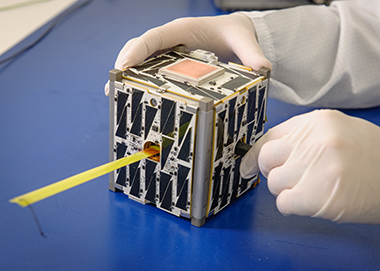
\includegraphics[scale = 2.5]{nanosat.jpg}
    \caption{A real life nanosat.}
\end{figure}
Current operating systems that are qualified for space missions are generally very costly. Consequently, general-purpose
OS-powered nanosat missions, such as Linux systems, have been deployed in the past. Leppinen \cite{b1} stated that choosing 
Linux limits the choice of hardware. Another major drawback is that Linux is not designed to be a real-time operating 
system. A real-time operating system is an OS that guarantees real-time applications a certain capability within a specified 
deadline. In some cases, design changes can reduce the number of challenging real-time applications. The remaining constraints 
require another dedicated controller to handle the real-time problem. 

% Background clarification
\section{Background}
The reliability of these OSs for a given hardware platform needs to be evaluated before their actual deployment.
Wali et al. \cite{b2} assessed the effects of the Linux OS on the fault tolerance of applications running on a RISC-V 
SoC(System on Chip) implemented in a Xilinx FPGA. To address the evaluation of the effects, we need to define the 
background. Although previous studies analyzed the fault tolerance of OS in embedded platforms, the following 
report will focus on radiation-induced configuration memory upsets on the reliability of applications running on 
a Linux RISC-V FPGA. Radiation-induced configuration memory upsets are a type of computer hardware failure caused 
by exposure to ionizing radiation from space. The radiation can create a charge that alters the state of a memory 
cell, causing a bit flip when the chip is exposed. It can result in errors in data storage or retrieval. In some
cases, it can crash the system. 
\subsection{FPGA Fault Injection} % Injection method
The method to simulate radiation-induced memory upsets is called FPGA fault injection. It is defined as the validation technique of fault-tolerant 
systems where the observation of the system's behavior in the presence of faults is done explicitly by 
injecting faults into the system. Reference \cite{b2} pointed out that FPGAs are an ideal fault-emulation platform 
due to their high logic density and reconfigurability. The FPGA consists of two layers, the user layer, and the configuration 
layer. Partially Modifying the configuration layer can start the injection process. Tawfeek et al. categorized the fault 
injection technique into three categories in \cite{b6}. In our case, we will be using software-based injection. 
The objective is to inject errors at the software level. The injected error simulates those that may occur due to hardware faults. 

% Experiment details
\section{Fault Injection Setup and Overview}
The hardware the experiment utilizes includes an Artix-7 series FPGA from Xilinx Inc. and a host computer. 
\subsection{Hardware Setup}
Figure 2 shows the block diagram of the hardware setup. 
The host PC is responsible for the fault injections and the debug software, which communicates with the FPGA's SoC
through a debug interface. The interface controls the executions of workload programs, collection of data, logging the errors,
and resets the program for the following execution. The workloads were tested both in bare-metal mode and with the Linux OS. 
Bare-metal mode runs directly on the hardware of a computer without any operating system or other software layers in between. 
\begin{figure}[ht]
    \centering
    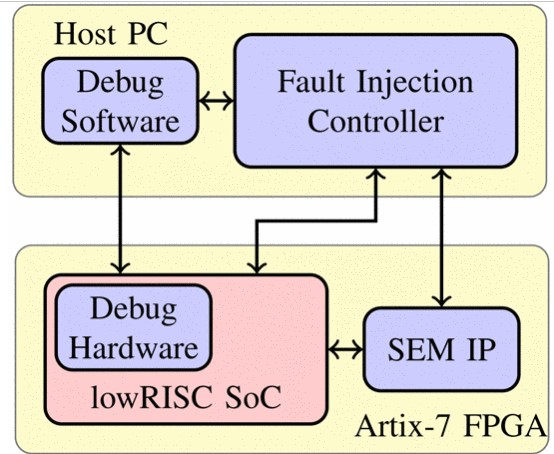
\includegraphics[scale = 0.5]{fault_inject.jpg}
    \caption{Block diagram of the fault injection setup.}
\end{figure}
The fault injection controller is located inside the host computer and utilizes Soft Error Mitigation Intellectual Property (SEM IP)
to introduce single event upsets (SEUs) into the Artix-7 FPGA's configuration memory. SEM IP includes hardware and software solutions 
that can detect and correct soft errors in real-time, and an SEU is a type of soft error that occurs when an electronic system is 
exposed to high-energy particles or radiation. Maillard et al. from Xilinx performed a similar analysis\cite{b5} to simulate the 
impact of radiation on the FPGA, but they utilized a proton beam rather than actual radiation.
\subsection{Benchmarks}
The workloads for fault injection consist of five mathematical algorithms: Tower of Hanoi, Dijkstra's algorithm, Matrix multiplication, 
Quick sort, and Merge sort. It is essential to know the Big-O(runtime complexities) of these algorithms because they can affect the fault 
injection results. Runtime complexity is a measure of how much time or space a program or algorithm takes to run as the input size increases. 
An algorithm with high runtime complexity is more vulnerable due to its increased complexity. It is also more difficult to identify the 
root cause of any observed failures. Figure 3 shows the Big-O of the algorithms. 
\begin{figure}[ht]
    \centering
    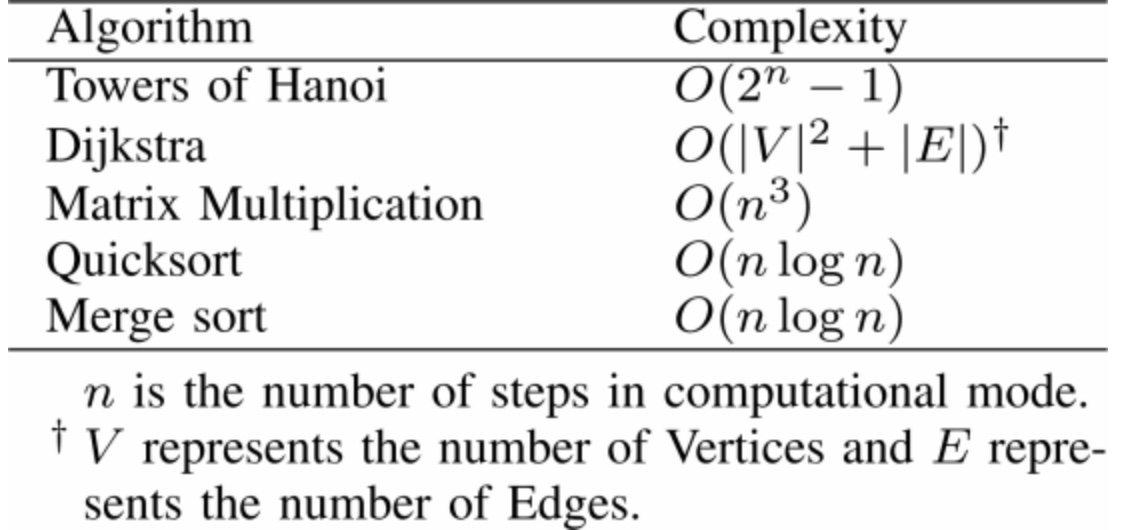
\includegraphics[scale = 0.17]{runtime.jpg}
    \caption{Workload's runtime complexity.}
\end{figure}
\subsection{Fault Models}
There are a total of 10 fault injection campaigns in the experiment, and each campaign is carried out on 5 distinct workloads. Each fault injection 
campaign injects bit-flips in 10,000 randomly selected essential bits in the memory. Faults are only injected in the configuration memory because
it accounts for most of the on-chip memory, which is large enough that it is very sensitive to SEUs. This fault model has been proven in detail
by \cite{b3}. 

% Results analysis
\section{Results Analysis}
After the fault injection campaigns, the error log is categorized into the following categories:
\begin{itemize}
    \item Masked: an error that is hidden or suppressed by other processes or software layers 
    \item Silent data corruption(SDC): data errors that occur without any visible symptoms or error messages
    \item Crash: an unexpected and abrupt termination of a software program due to an error/exception that stopped functioning
    \item Hang: a state where a software program becomes unresponsive and stops processing 
    \item Architectural Internal Failure(AIF): a software failure that occurs due to a flaw or error in the design or architecture of the software system itself
\end{itemize}
Crashes and Hangs are single-event functional interrupts, so a system reset was required to resume operation. SDCs and AIFs are tolerated in 
consumer electronics but are labeled as reliability threats in safety-critical systems. 

50,000 injections were performed in total. The results of the injections are shown in Figures 4(a) and 4(b). Each bar represents the percentage 
of errors encountered in each of the categories in the error log. 
\begin{figure}[ht]
    \centering
    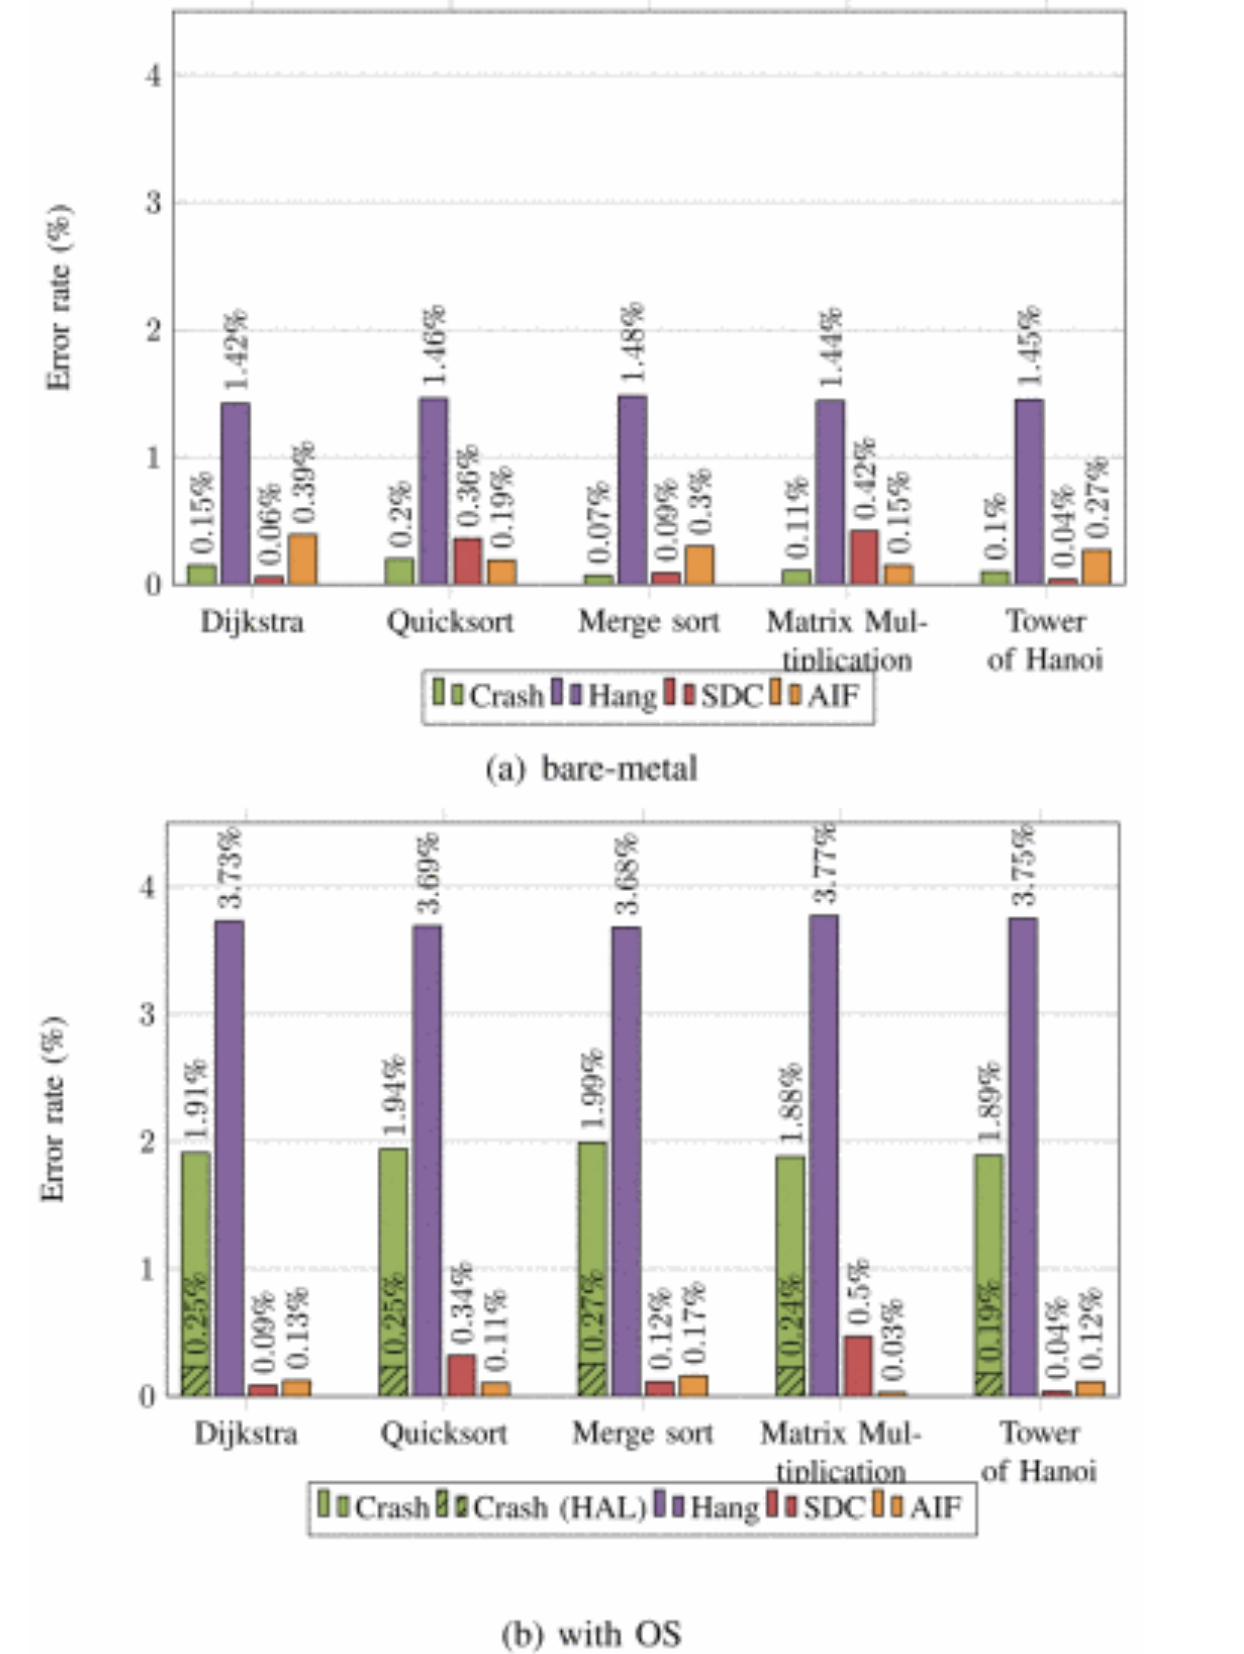
\includegraphics[scale = 0.2]{results.jpg}
    \caption{Error frequencies of the algorithms.}
\end{figure}
The percentages of crashes and hangs show consistency between benchmarks on both bare-metal and with Linux OS. This shows that upsets are 
primarily caused by the control functionality, not the fault injections. However, SDCs and AIFs vary between benchmarks in both scenarios. 
This suggests that the faults actually caused damage to the data. 

Hangs occurred the most in both bare-metal mode and with the Linux OS. The main difference is that the error rate with the OS is 
approximately 2.6 times higher than with bare-metal mode. Additionally, crashes have the highest percentage in each benchmark in both categories. 
The chances of crashes are 17.4 times higher when the Linux OS is present. There are numerous causes why the rates are significantly higher for
hangs and crashes. First, the Linux operating system is designed to support a wide range of hardware and software components, which can introduce 
compatibility issues with the FPGA hardware. Second, running Linux uses a kernel and drivers, which adds a layer of complexity to the system. 
Third, Linux uses a virtual memory system that requires hardware support from the FPGA, and implementing this correctly can be challenging, and 
errors can lead to system instability.

Fewer AIFs appeared with Linux OS for all benchmark workloads. The reason is that some memory upsets affecting the processor memory 
may be flagged by the OS as problems and resulted in crashes rather than AIFs. SDCs primarily depends on the design and implementation of the error 
detection and correction mechanisms. Similarly, the OS does not increase the SDC rate. In \cite{b7}, Santini et al. also proved that the SDC 
rate is barely affected by the presence of Linux. Additionally, \cite{b4} goes into detail on why Linux does not significantly impact the SDC rate. 

% Conclusion
\section{Conclusion}
In conclusion, the open-source and the ease of configuration nature of RISK-V FPGAs have made them a popular choice among developers. 
The use of these FPGAs in nanosats is also gaining attraction. As a result, it is crucial to evaluate their reliability under extreme 
circumstances. This report examined the impact of the Linux operating system on the reliability of RISC-V-based FPGAs compared 
to bare metal mode. Through the use of fault injections to simulate the radiation effects on FPGAs, we gained more understanding of 
the difference between a Linux-run FPGA compared to a bare metal RISC-V-based FPGA. 

% Citations
\begin{thebibliography}{10}
    \bibitem{b1} H. Leppinen, "Current use of linux in spacecraft flight software," in IEEE Aerospace and Electronic Systems Magazine,
    vol. 32, no. 10, pp. 4-13, October 2017, doi: 10.1109/MAES.2017.160182. 
    \bibitem{b2} I. Wali, A. Sánchez-Macián, A. Ramos and J. A. Maestro, "Analyzing the impact of the Operating System on the Reliability
    of a RISC-V FPGA Implementation," 2020 27th IEEE International Conference on Electronics, Circuits and Systems (ICECS), Glasgow, UK, 2020,
    pp. 1-4, doi: 10.1109/ICECS49266.2020.9294858.
    \bibitem{b3} L. Sterpone and M. Violante, "A New Partial Reconfiguration-Based Fault-Injection System to Evaluate SEU Effects in SRAM-Based
    FPGAs," in IEEE Transactions on Nuclear Science, vol. 54, no. 4, pp. 965-970, Aug. 2007, doi: 10.1109/TNS.2007.904080.
    \bibitem{b4} P. Bodmann, G. Papadimitriou, D. Gizopoulos and P. Rech, "Impact of Cores Integration and Operating System on ARM Processors 
    Reliability: Micro-Architectural Fault-Injection vs Beam Experiments," 2020 20th European Conference on Radiation and Its Effects on 
    Components and Systems (RADECS), Toulouse, France, 2020, pp. 1-4, doi: 10.1109/RADECS50773.2020.9857727.
    \bibitem{b5} P. Maillard et al., "Single-Event Evaluation of Xilinx 16nm UltraScale+™ Single Event Mitigation IP," 2018 IEEE Radiation 
    Effects Data Workshop (REDW), Waikoloa, HI, USA, 2018, pp. 1-5, doi: 10.1109/NSREC.2018.8584298.
    \bibitem{b6} R. M. Tawfeek, M. G. Egila, Y. Alkabani and I. M. Hafez, "Fault injection for FPGA applications in the space," 2017 12th
    International Conference on Computer Engineering and Systems (ICCES), Cairo, Egypt, 2017, pp. 390-395, doi: 10.1109/ICCES.2017.8275338.
    \bibitem{b7} T. Santini, L. Carro, F. Rech Wagner and P. Rech, "Reliability Analysis of Operating Systems and Software Stack for Embedded 
    Systems," in IEEE Transactions on Nuclear Science, vol. 63, no. 4, pp. 2225-2232, Aug. 2016, doi: 10.1109/TNS.2015.2513384.
\end{thebibliography}

\end{document}
